% Fig. 1 -- SCALE layered architecture (five processing layers + persistent data store)
\documentclass[tikz,border=6pt]{standalone}
\usepackage{mathptmx}
\usetikzlibrary{arrows.meta,positioning,calc,fit}
\definecolor{l1f}{HTML}{E8E8FF}\definecolor{l1b}{HTML}{6666FF}
\definecolor{l2f}{HTML}{FFF3E6}\definecolor{l2b}{HTML}{FFA940}
\definecolor{l3f}{HTML}{E9FFE9}\definecolor{l3b}{HTML}{00A000}
\definecolor{l4f}{HTML}{F5E9F5}\definecolor{l4b}{HTML}{B040B0}
\definecolor{l5f}{HTML}{E8F3F3}\definecolor{l5b}{HTML}{60B0B0}
\begin{document}
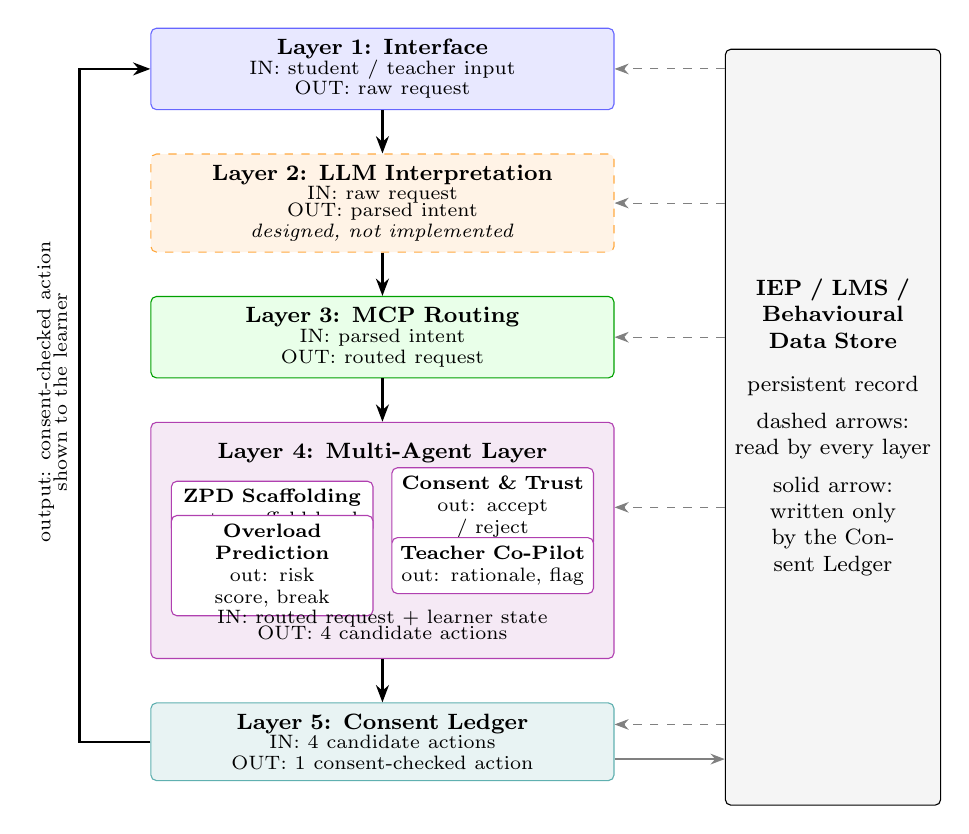
\begin{tikzpicture}[
  font=\footnotesize,
  layer/.style={draw,rounded corners=2pt,align=center,text width=5.6cm,inner sep=4pt},
  agent/.style={draw=l4b,fill=white,rounded corners=2pt,align=center,text width=2.35cm,inner sep=3pt,font=\scriptsize},
  down/.style={-{Stealth[length=2.2mm]},thick},
  rd/.style={-{Stealth[length=1.8mm]},dashed,gray}]
\node[layer,draw=l1b,fill=l1f] (L1) at (0,0) {\textbf{Layer 1: Interface}\\[-1pt]{\scriptsize IN: student / teacher input\\[-2pt] OUT: raw request}};
\node[layer,draw=l2b,fill=l2f,dashed,below=0.55cm of L1] (L2) {\textbf{Layer 2: LLM Interpretation}\\[-1pt]{\scriptsize IN: raw request\\[-2pt] OUT: parsed intent\\[-2pt] \textit{designed, not implemented}}};
\node[layer,draw=l3b,fill=l3f,below=0.55cm of L2] (L3) {\textbf{Layer 3: MCP Routing}\\[-1pt]{\scriptsize IN: parsed intent\\[-2pt] OUT: routed request}};
\node[layer,draw=l4b,fill=l4f,below=0.55cm of L3,minimum height=3.0cm,anchor=north] (L4) {};
\node[anchor=north] at ($(L4.north)+(0,-0.15)$) {\textbf{Layer 4: Multi-Agent Layer}};
\node[agent] (a1) at ($(L4.center)+(-1.4,0.42)$) {\textbf{ZPD Scaffolding}\\out: scaffold level};
\node[agent] (a2) at ($(L4.center)+(1.4,0.42)$) {\textbf{Consent \& Trust}\\out: accept / reject};
\node[agent] (a3) at ($(L4.center)+(-1.4,-0.32)$) {\textbf{Overload Prediction}\\out: risk score, break};
\node[agent] (a4) at ($(L4.center)+(1.4,-0.32)$) {\textbf{Teacher Co-Pilot}\\out: rationale, flag};
\node[anchor=south,font=\scriptsize,align=center] at ($(L4.south)+(0,0.12)$) {IN: routed request + learner state\\[-2pt] OUT: 4 candidate actions};
\node[layer,draw=l5b,fill=l5f,below=0.55cm of L4] (L5) {\textbf{Layer 5: Consent Ledger}\\[-1pt]{\scriptsize IN: 4 candidate actions\\[-2pt] OUT: 1 consent-checked action}};
\foreach \a/\b in {L1/L2,L2/L3,L3/L4,L4/L5} \draw[down] (\a.south)--(\b.north);
% data store
\node[draw,rounded corners=2pt,fill=gray!8,align=center,text width=2.5cm,minimum height=9.6cm,anchor=west]
  (DS) at ($(L1.east)+(1.4,-4.55)$) {\textbf{IEP / LMS /\\Behavioural\\Data Store}\\[6pt]{\footnotesize persistent record}\\[4pt]{\footnotesize dashed arrows:\\ read by every layer}\\[4pt]{\footnotesize solid arrow:\\ written only by the Consent Ledger}};
\foreach \n in {L1,L2,L3} \draw[rd] (DS.west |- \n.east) -- (\n.east);
\draw[rd] ($(DS.west |- L5.east)+(0,0.22)$) -- ($(L5.east)+(0,0.22)$);
\draw[rd] (DS.west |- a2.east) -- (L4.east |- a2.east);
\draw[-{Stealth[length=1.8mm]},gray,thick] ($(L5.east)+(0,-0.22)$) -- ($(L5.east -| DS.west)+(0,-0.22)$);
% feedback loop
\draw[-{Stealth[length=2.2mm]},thick] (L5.west) -- ++(-0.9,0) |- (L1.west);
\node[rotate=90,font=\scriptsize,align=center] at ($(L1.west)+(-1.25,-4.1)$) {output: consent-checked action\\[-2pt] shown to the learner};
\end{tikzpicture}
\end{document}
